\section*{Результаты измерений}

\begin{wrapfigure}{r}{0.3 \textwidth}
	\centering
	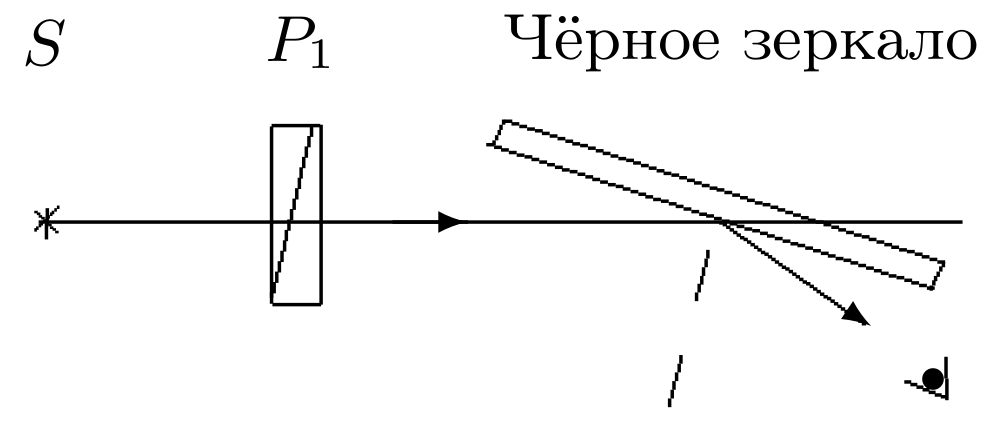
\includegraphics[width=0.28\textwidth]{../Изображения/black mirror.png}
\end{wrapfigure}

1. С помощью метода чёрного зеркала было определено разрешённое направление первого поляроида $\varphi_1 = 87^{\circ} \pm 1^{\circ}$. Поляроид пропускает свет, плоскость колебаний которого горизонтальная.

С помощью первого поляроида было определено разрешённое направление второго поляроида $\varphi_2 = 115^\circ \pm 1^{\circ}$. Поляроид пропускает свет, плоскость колебаний которого вертикальная.

2. Определим показатель преломления эбонита по формуле:
$$
n = \tg \varphi_Б
$$
Угол Брюстера без светофильтра $\varphi_{Б1} = 52^\circ \pm 3^\circ$. \\
Угол Брюстера со светофильтром $\varphi_{Б2} \in [46^\circ \pm 3^\circ; 54^\circ \pm 3^\circ]$.

$n_1 = 1,28 \pm 0,13$ \\
$n_2 \in [1,04 \pm 0,10; 1,38 \pm 0,14]$.

Погрешность косвенных измерений оценим по формуле:
$$
\sigma_n = \frac{\partial n}{\partial \varphi} \sigma_\varphi = \frac{\sigma_\varphi}{\cos^2 \varphi}
$$

Табличное значение показателя преломления эбонита $n_{табл} = 1,6 \div 1,7$.

Расхождение табличных и экспериментальных значений показателя преломления скорее всего связано с неточностью определения угла Брюстера, так как минимальная интенсивность определялась на глаз.

\begin{wrapfigure}{r}{0.3 \textwidth}
	\centering
	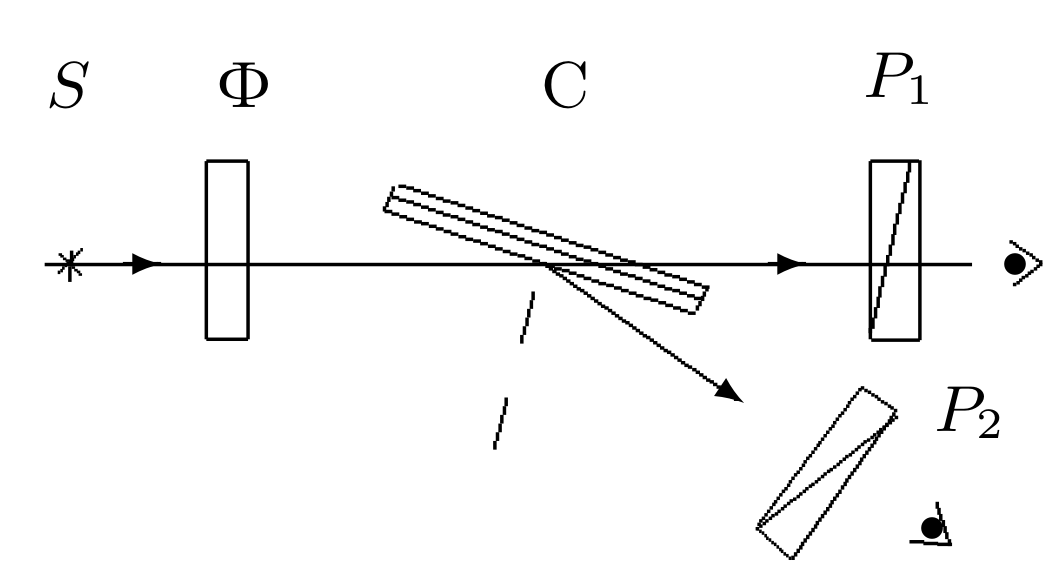
\includegraphics[width=0.28\textwidth]{../Изображения/glass stack.png}
\end{wrapfigure}

3. Исследуем поляризационные свойства стопы стеклянных пластин при падении неполяризованного света под углом Брюстера.

Для света, прошедшего стопу стеклянных пластин, интенсивность горизонтальной компоненты больше интенсивности вертикальной.

У света отражённого от стопы стеклянных пластин горизонтальная компонента практически отсутствует, а вертикальная компонента хорошо видна.

Интенсивность вертикальной компоненты отражённого от стопы стеклянных пластин света больше интенсивности вертикальной компоненты прошедшего света.

\begin{wrapfigure}{r}{0.3 \textwidth}
	\centering
	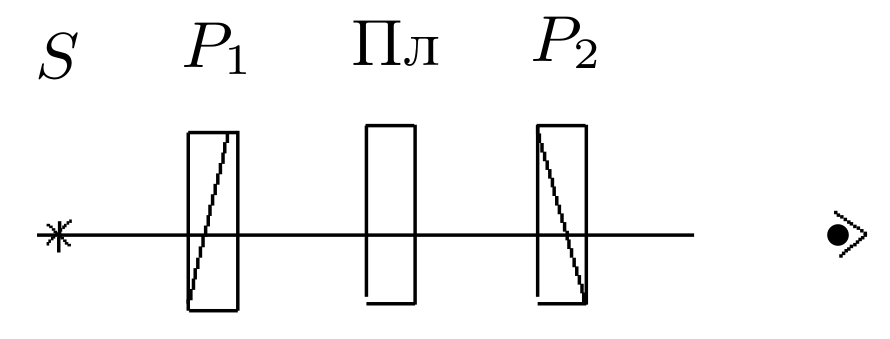
\includegraphics[width=0.28\textwidth]{../Изображения/main directions.png}
\end{wrapfigure}

4. Определим главные направления двоякопреломляющих пластин.

Пластина <<2 в кружочке>>. Направления наименьшей интенсивности: \\
$\varphi_{11} = 16^\circ$. \\
$\varphi_{12} = 110^\circ$. \\
$\varphi_{13} = 196^\circ$. \\
$\varphi_{14} = 288^\circ$. \\

Пластина <<2>>. \\
$\varphi_{11} = 40^\circ$. \\
$\varphi_{12} = 130^\circ$. \\
$\varphi_{13} = 220^\circ$. \\
$\varphi_{14} = 310^\circ$. \\

5. Добавим к схеме для определения главных направлений зелёный фильтр и повернём главные направления исследуемых пластин на $45^\circ$ вокруг главной оптической оси системы, оба поляроида установим в горизонтальное положение пропускания. Если исследуемая пластина $\frac{\lambda}{2}$, то сквозь систему свет проходить не будет.

В результате эксперимента определили, что пластина <<2>> -- пластина $\frac{\lambda}{2}$ -- на выходе создаёт линейную поляризацию, пластина <<2 в кружочке>> -- пластина $\frac{\lambda}{4}$ -- на выходе создаёт эллиптическую поляризацию.

6. С помощью пластинки чувствительного оттенка в $\lambda$ определили, что оси $\varphi_0 = 155^\circ$ соответствует большая скорость распространения, так как в этом случае проходящий систему свет приобретает голубую окраску. В перпендикулярном направлении окраска проходящего света -- оранжевая.

7. Исследуем интерференцию поляризованных лучей. Разместим между скрещенными поляроидами мозаичную слюдяную пластинку, собранную из 4 узких полосок слюды, лежащих по сторонам квадрата (две полоски $\frac{\lambda}{4}$, одна $\frac{\lambda}{2}$ и ещё одна $\frac{3\lambda}{4}$). В центре слюды нет, главные направления пластинок ориентированы параллельно сторонам квадрата.

Наблюдаемые картины при вращении поляроида $P1$ при неизменном $P2$.

\begin{figure}
	\centering
	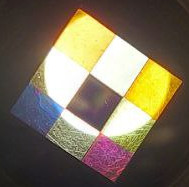
\includegraphics[width=0.3\textwidth]{../Изображения/1.jpg}
\end{figure}

\begin{figure}
	\centering
	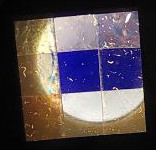
\includegraphics[width=0.3\textwidth]{../Изображения/2.jpg}
	\caption{На фотографии квадраты видны, как окрашены в синий, при наблюдении глаз воспринимал этот цвет как чёрный.}
\end{figure}

\begin{figure}
	\centering
	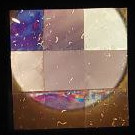
\includegraphics[width=0.3\textwidth]{../Изображения/3.jpg}
	\caption{На фотографии квадраты видны, как окрашены в синий, при наблюдении глаз воспринимал этот цвет как чёрный.}
\end{figure}

Наблюдаемые картины при вращении поляроида $P2$ при неизменном $P1$.

\begin{figure}
	\centering
	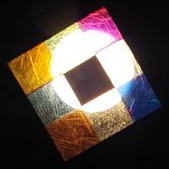
\includegraphics[width=0.3\textwidth]{../Изображения/4.jpg}
\end{figure}

\begin{figure}
	\centering
	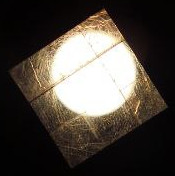
\includegraphics[width=0.3\textwidth]{../Изображения/5.jpg}
\end{figure}

\begin{figure}
	\centering
	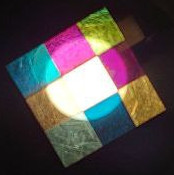
\includegraphics[width=0.3\textwidth]{../Изображения/6.jpg}
	\caption{Глаз зелёный верхний квадрат и оранжевый правый видел как прозрачные.}
\end{figure}

8. В работе было определено направление вращения эллиптически поляризованной волны -- правая поляризация.